%% Based on a TeXnicCenter-Template by Tino Weinkauf.
%%%%%%%%%%%%%%%%%%%%%%%%%%%%%%%%%%%%%%%%%%%%%%%%%%%%%%%%%%%%%

%%%%%%%%%%%%%%%%%%%%%%%%%%%%%%%%%%%%%%%%%%%%%%%%%%%%%%%%%%%%%
%% HEADER
%%%%%%%%%%%%%%%%%%%%%%%%%%%%%%%%%%%%%%%%%%%%%%%%%%%%%%%%%%%%%
\documentclass[letterpaper,oneside,10pt]{article}
% Alternative Options:
%	Paper Size: a4paper / a5paper / b5paper / letterpaper / legalpaper / executivepaper
% Duplex: oneside / twoside
% Base Font Size: 10pt / 11pt / 12pt


%% Language %%%%%%%%%%%%%%%%%%%%%%%%%%%%%%%%%%%%%%%%%%%%%%%%%
\usepackage[USenglish]{babel} %francais, polish, spanish, ...
\usepackage[T1]{fontenc}
\usepackage[ansinew]{inputenc}

\usepackage{lmodern} %Type1-font for non-english texts and characters


%% Packages for Graphics & Figures %%%%%%%%%%%%%%%%%%%%%%%%%%
\usepackage{graphicx} %%For loading graphic files
%\usepackage{subfig} %%Subfigures inside a figure
%\usepackage{pst-all} %%PSTricks - not useable with pdfLaTeX

%% Please note:
%% Images can be included using \includegraphics{Dateiname}
%% resp. using the dialog in the Insert menu.
%% 
%% The mode "LaTeX => PDF" allows the following formats:
%%   .jpg  .png  .pdf  .mps
%% 
%% The modes "LaTeX => DVI", "LaTeX => PS" und "LaTeX => PS => PDF"
%% allow the following formats:
%%   .eps  .ps  .bmp  .pict  .pntg


%% Math Packages %%%%%%%%%%%%%%%%%%%%%%%%%%%%%%%%%%%%%%%%%%%%
\usepackage[leqno]{amsmath}
%\usepackage{amsthm}
%\usepackage{amsfonts}


%% Line Spacing %%%%%%%%%%%%%%%%%%%%%%%%%%%%%%%%%%%%%%%%%%%%%
%\usepackage{setspace}
%\singlespacing        %% 1-spacing (default)
%\onehalfspacing       %% 1,5-spacing
%\doublespacing        %% 2-spacing


%% Other Packages %%%%%%%%%%%%%%%%%%%%%%%%%%%%%%%%%%%%%%%%%%%
%\usepackage{a4wide} %%Smaller margins = more text per page.
%\usepackage{fancyhdr} %%Fancy headings
%\usepackage{longtable} %%For tables, that exceed one page


%%%%%%%%%%%%%%%%%%%%%%%%%%%%%%%%%%%%%%%%%%%%%%%%%%%%%%%%%%%%%
%% Remarks
%%%%%%%%%%%%%%%%%%%%%%%%%%%%%%%%%%%%%%%%%%%%%%%%%%%%%%%%%%%%%
%
% TODO:
% 1. Edit the used packages and their options (see above).
% 2. If you want, add a BibTeX-File to the project
%    (e.g., 'literature.bib').
% 3. Happy TeXing!
%
%%%%%%%%%%%%%%%%%%%%%%%%%%%%%%%%%%%%%%%%%%%%%%%%%%%%%%%%%%%%%

%%%%%%%%%%%%%%%%%%%%%%%%%%%%%%%%%%%%%%%%%%%%%%%%%%%%%%%%%%%%%
%% Options / Modifications
%%%%%%%%%%%%%%%%%%%%%%%%%%%%%%%%%%%%%%%%%%%%%%%%%%%%%%%%%%%%%

%\input{options} %You need a file 'options.tex' for this
%% ==> TeXnicCenter supplies some possible option files
%% ==> with its templates (File | New from Template...).



%%%%%%%%%%%%%%%%%%%%%%%%%%%%%%%%%%%%%%%%%%%%%%%%%%%%%%%%%%%%%
%% DOCUMENT
%%%%%%%%%%%%%%%%%%%%%%%%%%%%%%%%%%%%%%%%%%%%%%%%%%%%%%%%%%%%%
\begin{document}

\pagestyle{empty} %No headings for the first pages.


%% Title Page %%%%%%%%%%%%%%%%%%%%%%%%%%%%%%%%%%%%%%%%%%%%%%%
%% ==> Write your text here or include other files.

%% The simple version:
\title{Empirical Analysis of Algorithms: Banker's Algorithm}
\author{Jessica Nguy \and Eric Pereira}
%\date{} %%If commented, the current date is used.
\maketitle
\newpage

%% The nice version:
%\input{titlepage} %%You need a file 'titlepage.tex' for this.
%% ==> TeXnicCenter supplies a possible titlepage file
%% ==> with its templates (File | New from Template...).


%% Inhaltsverzeichnis %%%%%%%%%%%%%%%%%%%%%%%%%%%%%%%%%%%%%%%
\tableofcontents %Table of contents
\cleardoublepage %The first chapter should start on an odd page.

\pagestyle{plain} %Now display headings: headings / fancy / ...



%% Abstract %%%%%%%%%%%%%%%%%%%%%%%%%%%%%%%%%%%%%%%%%%%%%%%%%

\begin{abstract}
This paper details the process of programming, profiling, analyzing, and writing of the group Empirical Analysis of Algorithms project. The project topic is Banker's Algorithm. The code itself is written with Visual Studio Code, the report is written with \LaTeX\ , and the profiler used is the GNU GProf.
\end{abstract}
\newpage

%% Section I : Problem %%%%%%%%%%%%%%%%%%%%%%%%%%%%%%%%%%%%%
\section{Problem}
Compute best time complexity and worst time complexity of the Banker's Algorithm.
\\
\\Let \textit{n} be the number of processes and \textit{m} be the number of resources.
\\The \textit{Claim Vector} is a data structure of size \textit{m} that determines the amount of available resources for each process. It is often referred to as \textit{Work}. \textit{Allocated Resources} is a data structure of size \textit{m*n} that determines the amount of resources assigned to each process. \textit{Maximum Claim} is an array of size \textit{m*n} that defines the maximum allowed resources that each process can use. \footnote{http://www.geeksforgeeks.org/operating-system-bankers-algorithm/}
\\The \textit{Need Matrix} is calculated from \textit{Allocated Matrix} and \textit{Maximum Claim}. It is calculated by $N[i][j] = M[i][j] - A[i][j]$.

%% Section II : Algorithm %%%%%%%%%%%%%%%%%%%%%%%%%%%%%%%%%%
\section{Algorithm}
The Safety Algorithm determines whether or not a system is in a $safe$ state. The system is considered $safe$ if all processes terminate. If processes do not terminate, then the system is in a deadlock and is considered $unsafe$.
\\
Safety Algorithm \\
\begin{quote}
	1.) Let Work and Finish be vectors of length \textit{m} and \textit{n} respectively.
	Initialize: $Work = Available$ \\
  Finish[\textit{i}] = $false$; for $i = 1, 2, ..., n$ \\ \\
	2.) Find an $i$ such that both \\
	a.) Finish[$i$] = $false$ \\
	b.) $Need_i$ \leq \textit{Work} \\
	If no such $i$ exists go to step (4) \\ \\
	3.) Work = Work + $Allocation_i$ \\
	\indent Finish[\textit{i}] = $true$ \\
	\indent Go to step (2) \\ \\
	4.) If Finish[\textit{i}] = $true$ for all \textit{i}, then the system is in $safe$ state \\
\end{quote}
\footnote{\url{http://www.geeksforgeeks.org/operating-system-bankers-algorithm/}}
The Resource-Request Algorithm allows for a process to 'request' for more resources so that it is able to terminate.
\begin{quotation}
Resource-Request Algorithm \\
	1.) If $Request_i$ $<$ $Need_i$ \\
					Go to step (2); otherwise raise an error condition, since the process has exceeded its maximum claim. \\ \\
	2.) If $Request_i$ $<$ $Available$ \\
					Go to step(3); otherwise $P_i$ must wait, since the resources are not available. \\ \\
	3.) Have the system pretend to have allocated the requested resources to process $P_i$ by modifying hte state as follows: \\ 
					$Available = Available - Request_i$ \\
					$Allocation_i = Allocation_i + Request_i$ \\
					$Need_i = Need_i - Request_i$ \\
\end{quotation} \footnote{http://www.geeksforgeeks.org/operating-system-bankers-algorithm/}
\\
\\
\subsection{Example}
Let $n = 3$ and $m = 4$.

The Claim Vector \textit{(W)} is:
\begin{left} \begin{tabular}{c c c c}
A & B & C & D	\\
\hline
3 & 1 & 1 & 2 \end{tabular}

The Allocated Resources \textit{(A)} is \begin{left} \begin{tabular}{c c c c}
A & B & C & D \\
\hline
1 & 2 & 2 & 1 \\
1 & 0 & 3 & 3 \\
1 & 2 & 1 & 0 \end{tabular}

The Maximum Claim \textit{(M)} is \begin{left} \begin{tabular}{c c c c}
A & B & C & D \\
\hline
3 & 3 & 2 & 2 \\
1 & 2 & 3 & 4 \\
1 & 3 & 5 & 0 \end{tabular}

\subsection{Safety Algorithm}
The program  determines whether or not the inputs are \textit{safe} or \textit{unsafe}. A program is considered $safe$ if all processes terminate. If the processes do not terminate and $W$ is smaller than all $P_n$ , then the operating system enters a deadlock and is considered as $unsafe$.\\
To calculate the Need Matrix (\textit{N}), we calculate $M[i][j] - A[i][j]$ for each index of the matrix.\\
Thus, the Need Matrix \textit{N} is \begin{left}\begin{tabular}{c c c c}
\\
A & B & C & D \\
\hline
2 & 1 & 1 & 1 \\
0 & 2 & 0 & 1 \\
0 & 1 & 4 & 0 \\
\end{tabular}
\\
\\

Iterate through the Need Matrix.
Given $i = 0$ we check if $N_0$ $<$ $W$
\begin{equation}
	$N_0 = <2 | 1 | 1 | 1> \\
	W 	 = <3 | 1 | 1 | 2>$ \\
	$N_0$ \leq $W$ 
\end{equation}
\\
Therefore, $N_0$ is less than $W$. Process 0 then terminates. Add the amount allocated to $P_0$ to the Claim Matrix.
\begin{equation}
	$W = W + A_0$ \\
	$<2 | 1 | 1 | 1> + <3 | 1 | 1 | 2> = <5 | 2 | 2 | 3>$
\end{equation}

Increase $i$ by 1 and continue until $i$ is equal to $n$.
\begin{equation}
	$N_1 = <0 | 2 | 0 | 1> \\
	W		 = <5 | 2 | 2 | 3>$ \\
	$N_1$ \leq $W$ 
\end{equation}
\\
$N_1$ is less than $W$. Process 1 then terminates. Add the amount allocated to $P_1$ to the Claim Matrix.
\begin{equation}
	$W = W + A_1$ \\
	$<5 | 2 | 2 | 3> + <1 | 0 | 3 | 3> = <6 | 2 | 5 | 6>$
\end{equation}
\\
Increase $i$ by 1 and continue until $i$ is equal to $n$.
\begin{equation}
	$N_2 = <1 | 3 | 5 | 0> \\
	W		 = <6 | 2 | 5 | 6>$ \\
	$N_2$ \leq $W$ 
\end{equation}
\\
$N_2$ is less than $W$. Process 2 then terminates. Add the amount allocated to $P_2$ to the Claim Matrix.
\begin{equation}
	$W = W + A_2$ \\
	$<6 | 2 | 5 | 6> + <1 | 3 | 5 | 0> = <7 | 5 | 10 | 6>$ \\
\end{equation}
End loop.
\\ 
\\
Therefore, since all processes terminated, the system is in a safe state. The order of processes that terminated is $P_0$, $P_1$, $P_2$.
If the \textit{Claim Matrix} was less than the \textit{Need Matrix}, skip the current process and return to it once the code has iterated through the loop once. If the process never terminates due to a lack of resources, then the system is in an unsafe state.

\subsection{Resource-Request Algorithm}
Process 2 requests resources of 1$B$ and 1$C$.
$R_2 = <0 | 1 | 1 | 0>$. Check if $R_2$ $<$ $N_2$.
\begin{equation}
	$R_2$ \leq $N_2$ \\
	<0 | 1 | 1 | 0> $<$ <0 | 1 | 4 | 0> 	
\end{equation}
$R_2$ is less than $N_2$. Proceed to step (2) of the Resource-Request Algorithm.
\\
Check if $R_2$ is less than the Available Resources ($W$).
\begin{equation}
	$R_2$ \leq $W$ \\
	<0 | 1 | 1 | 0> \leq <3 | 1 | 1 | 2> 	
\end{equation}
$R_2$ is less than $W$. Proceed to step (3) of the Resource-Request Algorithm.
\\
Calculate the new $W$, $A_2$, and $N_2$ line of the matrix.
\begin{equation}
	$W = W - R_2$\\
		 = <3 | 1 | 1 | 2> - <0 | 1 | 1 | 0>\\
		 = <3 | 0 | 0 | 2>\\
	\\
	$A_2 = A_2 + R_2$\\
			 = <1 | 2 | 1 | 0> + <0 | 1 | 1 | 0>\\
			 = <1 3 1 0>\\
	\\
	$N_2 = N_2 - R_2$\\
			 = <0 1 4 0> - <0 1 1 0>\\
		   = <0 0 3 0>
\end{equation}
\\
The Resource-Request Algorithm works for $P_2$ requesting $1B$ and $1C$. However, check with the Safety Algorithm to determine if this new request is safe for the operating system.
\begin{equation}
	i = 0 \\
		$N_0$ = <2 | 1 | 1 | 1> \\
		$N_0$ \leq $W$ \\
		<2 1 1 1> $>$ <3 0 0 2>
\end{equation}
	Since $N_0$ is not less than $W$, skip $P_0$ and increment $i$ by 1.
\begin{equation}
	i = 1 \\
		$N_1$ = <0 2 0 1> \\
		$N_1$ \leq $W$ \\
		<0 2 0 1> $>$ <3 0 0 2>
\end{equation}
	Since $N_1$ is not less than $W$, skip $P_1$ and increment $i$ by 1.
\begin{equation}
	i = 2 \\
		$N_2$ = <0 0 3 0> \\
		$N_2$ \leq $W$ \\
		<0 0 3 0> $>$ <3 0 0 2>
\end{equation}
\tab Since $N_2$ is not less than $W$, and that no processes have been terminated, the operating system enters into a deadlock. The process is an $unsafe$ state.

%% Section III : Implementation %%%%%%%%%%%%%%%%%%%%%%%%%%%%
\section{Implementation}
\tabThe algorithm is coded in C++ and prompts user input for \textit{n}, \textit{m}, \textit{Claim Vector}, \textit{Allocated Matrix}, and \textit{Maximum Claim}.

The code mostly features while- and for-loops to calculate the result of the algorithm.

\subsection{Code}
\footnote{\url{https://www.thecrazyprogrammer.com/2016/07/bankers-algorithm-in-c.html}} Code is based off of a C variant created by Neeraj Mishra. \textit{count} is equal to \textit{n}, so that the while loop has to run through at least \textit{n} loops (to go through each array size \textit{m}). \textit{running} array determines whether that specific array has already been reviewed, \textit{running} only holds 1 or 0 to determine true or false boolean var. \textit{max\_claim} subtracting the \textit{curr} ints at specific points in an array is equal to a specific point in the need matrix without creating the need matrix (this helped relieve some memory issues encountered when previously trying to store need matrix variables.)
\begin{verbatim}
while (count != 0) {
 safe = false;
  for (i = 0; i < p; i++) {
   if (running[i]) { 
    exec = 1;\\
    for (j = 0; j < r; j++) { 
     if (max_claim[i][j] - curr[i][j] > avl[j]) { 
      testNum = test(testNum); 
      exec = 0; 
      break; 
     } 
    } 
    if (exec) { 
     printf("\nProcess%d is executing.\n", i + 1);
      testNum = test(testNum);
      running[i] = 0;
      count--;
      safe = true;
      for (j = 0; j < r; j++)
       avl[j] += curr[i][j];
      break;
    }
   }
  }
  if (!safe) {
   printf("\nThe processes are in unsafe state.");
   break;
  }
  if (safe)
   printf("\nThe process is in safe state."); 
   printf("\nAvailable vector: "); 
   for (i = 0; i < r; i++)
    printf("%d ", avl[i]); 
}
\end{verbatim}

%% Section IV : Test %%%%%%%%%%%%%%%%%%%%%%%%%%%%%%%%%%%%%%%
\section{Test}
Was tested for best-case scenario and worst-case scenario. For best-case scenario, we had the \textit{Claim Vector} set to a large number, so that when the loop iterated through the \textit{Need Matrix}, the process would terminate, ensuring that the code iterates $n$ times. \\
\\Likewise to test the worst-case scenario, we set the \textit{Claim Vector} to a small number, so that the last process $P_n$ would terminate, then $P_n-1$ would terminate, and so on until $P_0$ terminates, ensuring that the code iterates $m*n$ times.

%% Section V : Profile %%%%%%%%%%%%%%%%%%%%%%%%%%%%%%%%%%%%%
\section{Profile}
\begin{center}
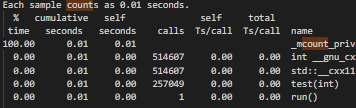
\includegraphics{bestcase.png}\\
\caption{Figure 1: Best time complexity Gprof chart for safe state\label{fig:fig1}}
\end{center}

\begin{center}
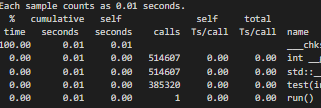
\includegraphics[scale]{worstcase.png}\\
\caption{Figure 2: Worst time complexity Gprof chart for safe state}
\end{center}

%% Section VI : Analyze %%%%%%%%%%%%%%%%%%%%%%%%%%%%%%%%%%%%
\section{Analyze}
The \textit{test} function is the function used the count calls. Gprof is a profiler that does not trace calls in a loop. In order to count how many times the algorithm was called upon the \textit{test} function was put in place as a dummy variable to check exactly how often it was called upon. 
\\
The chart produced in Figure 1 shows the best time complexity for a safe state algorithm that holds an \textit{n} value of 507, and an \textit{m} value of 507. Figure 1 shows that in best time case scenario it runs in \textit{nm} time as it runs 257,409 times. This produces a \( \Omega \)(n*m) time complexity.\\
\\
The chart produced by Gprof in figure 2 shows the worst time complexity for a safe state algorithm that holds the same \textit{n} and \textit{m} value as the best time complexity example. In this chart the test is called on 385,320 times, which is equal to:
\begin{equation}
\sum_{k=0}^{n-1} (m+k) = 385,320
\end{equation}
\\
This was the equation that was expected, This produces an O(n*n*m) time complexity. 
%% Section VII : Evaluate %%%%%%%%%%%%%%%%%%%%%%%%%%%%%%%%%%
\section{Evaluate}
%% Section VIII : Conclusions %%%%%%%%%%%%%%%%%%%%%%%%%%%%%%
The results that were expected were the results attained in our tests. According to the Algorithm, and predictions stated by the algorithm, there should be an \textit{n*m} calls to the test function in the best case scenario of a safe state run. This time complexity was expected as it would review \textit{n} processes and in each process do \textit{m} comparisons.  This is true according to the profiler, which shows that the algorithm is called on exactly \textit{n*m} times.\\
\\
According to our predictions as well worst case scenario would be \textit{n*n*m} calls to the test function. This is due to the \textit{Claim Vector} being called on and compared to every process array in the \textit{Need} matrix. That means going through \textit{n} arrays \textit{n} times, each array holding \textit{m} thus doing \textit{m} comparisons. This leaves with the equation number 13 specified in the Analyze portion. 
\section{Conclusions}
Banker's algorithm, although a good idea in theory, is not optimal in the use of operating systems, as it was initially built for. It is impossible for an operating system to always know how to make a possible \textit{need} matrix available for a program; however this deadlock avoidance system was found useful in banks as it prevented issues with bankruptcy and could be run to check, with absolute certainty, in the case that the \textit{need} matrix is absolutely certain and resources from the  \textit{max} matrix is malleable, as in there are resources that could eventually be moved out of it and it will not remain static.  

%%%%%%%%%%%%%%%%%%%%%%%%%%%%%%%%%%%%%%%%%%%%%%%%%%%%%%%%%%%%%
%% BIBLIOGRAPHY AND OTHER LISTS
%%%%%%%%%%%%%%%%%%%%%%%%%%%%%%%%%%%%%%%%%%%%%%%%%%%%%%%%%%%%%
%% A small distance to the other stuff in the table of contents (toc)
\addtocontents{toc}{\protect\vspace*{\baselineskip}}

%% The Bibliography
%% ==> You need a file 'literature.bib' for this.
%% ==> You need to run BibTeX for this (Project | Properties... | Uses BibTeX)
%\addcontentsline{toc}{chapter}{Bibliography} %'Bibliography' into toc
%\nocite{*} %Even non-cited BibTeX-Entries will be shown.
%\bibliographystyle{alpha} %Style of Bibliography: plain / apalike / amsalpha / ...
%\bibliography{literature} %You need a file 'literature.bib' for this.
\begin{thebibliography}{99}
\bibitem{gg} Banker's Algorithm \emph{Geeks for Geeks}, http://www.geeksforgeeks.org/operating-system-bankers-algorithm/ 
\bibitem{gg} Banker's Algorithm in C \emph{The Crazy Programer}, https://www.thecrazyprogrammer.com/2016/07/bankers-algorithm-in-c.html
\bibitem{gg} EWD 623: The mathematics behind the Banker's Algorithm, \emph{Edsger Dijkstra}, http://www.cs.utexas.edu/users/EWD/ewd06xx/EWD623.PDF 



%%%%%%%%%%%%%%%%%%%%%%%%%%%%%%%%%%%%%%%%%%%%%%%%%%%%%%%%%%%%%
%% APPENDICES
%%%%%%%%%%%%%%%%%%%%%%%%%%%%%%%%%%%%%%%%%%%%%%%%%%%%%%%%%%%%%
\appendix
%% ==> Write your text here or include other files.

%\input{FileName} %You need a file 'FileName.tex' for this.


\end{document}

